\chapter{Planning over Configuration Space Families}
\label{chap:family}

To this point,
we have considered motion planning problems in which a path is sought
within a fixed valid subset
$\mathcal{C}_{\ms{free}} \subset \mathcal{C}$
In Chapter~\ref{chap:lazysp},
we described a lazy search algorithm which is suited to domains in
which determining the weight of an edge
-- perhaps due to expensive set membership tests --
is expensive.
Chapter~\ref{chap:utility} discussed the concept of utility to
motion planning,
and showed examples of its application to single-query motion
planning problems.

However,
many applications exhibit structure beyond simple binary belief over
configuration validity.
In this chapter,
we introduce the \emph{family motion planning problem},
a generalization of the motion planning problem to a family of sets
over $\mathcal{C}$.
We then show how such a problem over familes can be represented
as in the utility function framework,
and given as input to the LEMUR motion planner described
in Chapter~\ref{chap:utility}.

This chapter proceeds as follows.
Section~\ref{sec:family:related-work} surveys related work.
In Section~\ref{sec:family:families-in-manipulation},
we motivate these the family motion planning problem
from the standpoint of manipulation tasks.
Section~\ref{sec:family:formulation} formulates the problem
generally.
We describe our approach in Section~\ref{sec:family:approach},
and Section~\ref{sec:family:as-utility} details how the family
problem can be represented as a utility function.
The remainder of the chapter examines several applications
of this decomposition,
such as multi-step geometry
(Section~\ref{subsec:family:app-multi-step})
and caching invariant geometry
(Section~\ref{subsec:family:cached-self-valid}),
conservative geometric approximations
(Section~\ref{subsec:family:broad-phase}),
and dynamic environments
(Section~\ref{subsec:family:dynamic-environments}).

\section{Related Work}
\label{sec:family:related-work}

The topic of reusing planning computation
between similar motion planning problems
has been extensively studied in the literature.
We include here a broad survey of existing approaches;
the application sections
(Section~\ref{subsec:family:app-multi-step}
-- \ref{subsec:family:dynamic-environments}) also include
relevant references to prior work.

\paragraph{Exact Algorithms.}
Exact planning methods construct explicit obstacles
directly in the configuration space.
Many such approaches allow for precomputation of primitives,
such as bitmaps \citep{kavraki1995cspacefft}
or C-space primitives for different workspace obstacles
\citep{newmanbranicky1991cspacetransforms}.
More recently,
Lien and Lu \citep{lien2009similarobstacles} describe a method to
build a PRM around obstacles in a database,
and then reposes them in a new world.
As described in Section~\ref{subsec:roadmaps:sensitive},
the exact approach is not easily applicable to articulated robots
with complex mappings from workspace to C-space.

\paragraph{Accommodating Dynamic Subsets in Sampling-Based Planning.}
Strong recent interest in sampling-based planning
has lead to the development of a number of approaches to handle
environments in which $\mathcal{C}_{\ms{free}}$ changes over time.
If a given discretization is asserted a priori,
this problem setting is similar to the dynamic shortest path problem
from Chapter~\ref{chap:ibid};
we refer the reader to that chapter for a review of related work.
Many sampling-based approaches attempt to prune and grow
the discretizations itself in response to these changes,
such as the Dynamic RRT \citep{ferguson2006drrt},
the Reconfigurable Random Forest (RRF)
\citep{li2002incrementalprmmanagement},
and the Lazy Reconfiguration Forest
\citep{gayle2007lazyreconfigforest}.
%We do the lazy thing as well (built into our planner).
%None of these reason about the structure of the configuration space.
However, these approaches do not reason explicitly about the
structure of the configuration space,
which we will consider
in Section~\ref{sec:family:families-in-manipulation}.

\paragraph{Considering Static and Dynamic Obstacles Separately.}
Some approaches do take advantage of such structure
through a two-level dichotomy between
the \emph{permanent} and \emph{non-permanent} configuration space
obstacles that induce $\mathcal{C}_{free}$.
Leven and Hutchinson \citep{leven2000changing}
and similar work \citep{kallman2004dynamicroadmaps}
handle changing environments by
precomputing a self-collision-free roadmap offline,
and then pruning it at query time
using a mapping from workspace cells to roadmap edges.
%This can also be viewed through the multi-space lens
%-- I think this is just an instantiation of a bunch of sets.
%They're very focused on the precomputation stuff.
%However, this approach this can't directly handle grasped objects.
Other methods \citep{jaillet2004dynamicprm}
exploit the dichotomy between static and dynamic parts of
the world online.

\paragraph{Task and Motion Planning.}
The structure in manipulation tasks that our approach leverages
is similar to the \emph{conditional reachability graph} which is
part of the recent \textsc{FFRob} heuristic task planning framework
\citep{garrett2014ffrob}.
While this framework does make use of a similar configuration
space decomposition for manipulation tasks
as described in Section~\ref{sec:family:families-in-manipulation},
it differs from our approach in two ways.
First,
it is concerned only with manipulation tasks,
and does not consider how the induced set of motion planning problems
can be formulated more generally
(e.g. in Section~\ref{sec:family:formulation}).
Second,
because the framework does not consider utility,
its motion planner is not able to exploit the configuration space
structure to the same extent as our approach.

%\subsection{Fast Collision Checking}
%
%Broad-phase collision checking.
%See Section~\ref{subsec:broad-phase} for more on this.
%I need cites!

%\subsection{Sampling Strategies}
%
%Also Kurniawati and Hsu's
%\emph{Workspace-based Connectivity Oracle}
%\citep{kurniawati2008workconnoracle}
%which is a smart sampling strategy which considers workspace
%geometry to inform PRM sampling.
%Kurniawati has a bunch of other work on PRM fundamentals and sampling.
%I think our approach is complementary to a PRM sampling strategy.
%Or, you could do deterministic sampling
%\citep{lavalle2002gridprms} \citep{geraerts2002prmcomparison}.
%
%\subsection{Multi-Resolution Planning}
%
%\noindent
%\begin{itemize}
%\item S. Kambhampati 1986
%\item R. Steffens 2010
%\item S. Zickler 2010
%\item K. Gochev 2013
%\end{itemize}

%\subsection{Graph Search}

%Many graph-search approaches are relevant to planning in similar
%environments.
%Algorithms such as
%D* \citep{stentz1994dstar}
%or LPA* \citep{koenig2004lpastar}
%handle dynamically changing (or incrementally discovered) worlds.
%Experience graphs \citep{phillips2012egraphs} are a method to apply
%computation from previous graph-search planning queries
%to the current problem.

%\subsection{Other Related Work to Integrate}
%
%Symbolic planning frameworks.

\section{Motivation: Families in Manipulation Tasks}
\label{sec:family:families-in-manipulation}

Motion planning approaches that build graphs
in the collision-free subset of
configuration space as described in Chapter~\ref{chap:roadmaps},
e.g. the
PRM \citep{kavrakietal1996prm}
and RRT \citep{lavallekuffner1999rrt},
have proven promising
for high-dimensional articulated robotics problems
in unstructured environments.
These approaches devote a large amount of computational effort
testing configurations and paths for collision
via the free set indicator function
(Section~\ref{subsec:roadmaps:building-graphs}),
and multi-query planners can then reuse the resulting graph
for other queries in the same collision-free subset.

However,
for manipuation problems,
this subset of the robot's configuration space
is sensitive to the locations and shapes of
both people and objects in the environment,
as well as the robot itself.
It also depends on the shape and pose of any object
grasped by the robot.
Consider the table clearing task in
Figure~\ref{fig:family:herbbin-multistep-example}.
The robot's valid subset $\mathcal{C}_{\ms{free}}$
changes each time the object is grasped or released.
Over the course of a planning episode,
these changing subsets constitute a family of related sets over
$\mathcal{C}$.

\begin{marginfigure}
   \centering
   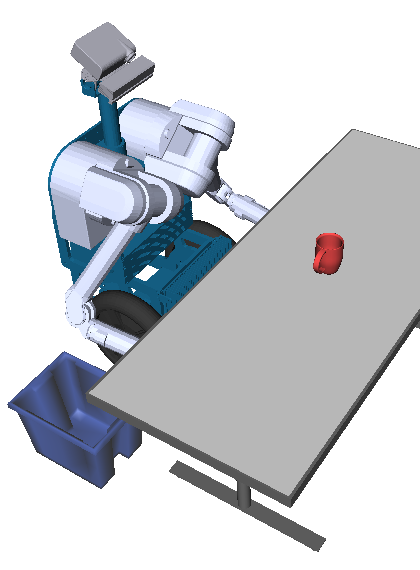
\includegraphics[width=2.5cm]{figs/herbbin/step0cropped.png}%
   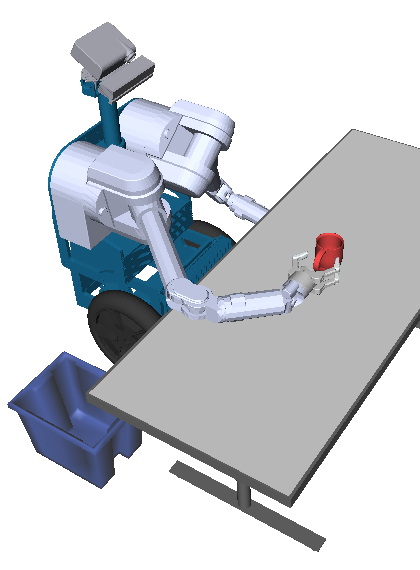
\includegraphics[width=2.5cm]{figs/herbbin/step01cropped.png}

   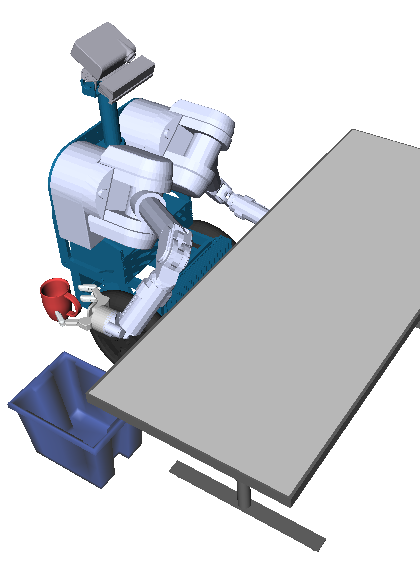
\includegraphics[width=2.5cm]{figs/herbbin/step12cropped.png}%
   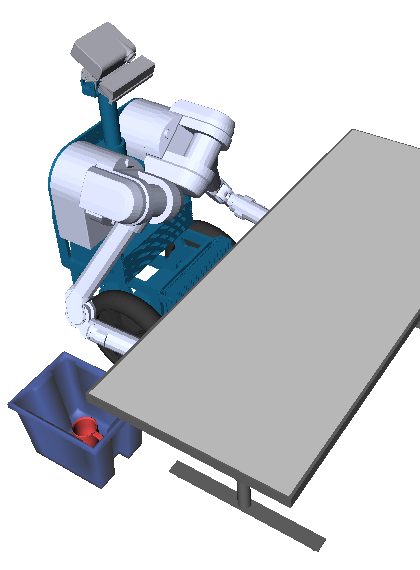
\includegraphics[width=2.5cm]{figs/herbbin/step2cropped.png}

   \caption{A simple manipulation task: retreive the mug from
      the table, and drop it in the blue bin.
      This task requires plans in three distinct C-space free subsets.}
   \label{fig:family:herbbin-multistep-example}
\end{marginfigure}

This makes it difficult not only to apply the results of prior
planning computation to the current problem,
but also to efficiently consider multiple planned or hypothesized
motions,
since we must reconstruct our graph from scratch whenever
the environment changes.
This is especially the case for
multi-step manipulation tasks that must be planned into the future.
%We want to continuously update our representation for detours.

We use this multi-step manipulation task as a motivating example
for the family motion planning problem,
and dive more deeply next into the structure of the problem's
composite configuration space.
We will consider problems over other robots and applications
later in this chapter.

\subsection{The Composite Configuration Space}

The configuration of a quasistatic manipulation environment
with multiple moveable objects can be represented as a
\emph{composite configuration space},
\marginnote{The composite configuration space is also called
the \emph{joint configuration space}.}
consisting of the Cartesian product of the individual configuration
spaces of the constituent objects.
For example,
consider an environment with a robot $R$ and an object $O$;
each is endowed with a configuration space:
\begin{equation}
   \mathcal{C}_R \quad\mbox{and}\quad \mathcal{C}_O.
\end{equation}
For example,
the robot's configuration space may be represented as its joint angles,
while the object's configuration may be $SE(3)$.
The composite space is then defined as
\begin{equation}
   \mathcal{C}_{RO} = \mathcal{C}_R \times \mathcal{C}_O.
\end{equation}
Of course,
not all composite configurations will be feasible;
some may correspond to configurations in which the robot,
object, or static environment are intersecting each other (colliding),
while others may denote configurations of the object where it is
not at a stable placement or grasp configuration.

\paragraph{Visualizating the Composite Configuration Space.}
While the composite configuration space for any interesting
manipulation task
is of too high dimension to effectively visualize in full,
we can make an approximation shown
in Figure~\ref{fig:family:composite-volumes}.
Imagine that this 3D visualization represents a projection of
$\mathcal{C}_{RO}$
so that the two horizontal axes $x$ and $y$ correspond to
the robot's configuration space $\mathcal{C}_{R}$,
while the vertical axis $z$ corresponds to the object's
configuration space $\mathcal{C}_{O}$.
For the sake of this visualization,
we ignore constraints on feasible object placements.

\begin{figure}
   \centering
   \begin{tikzpicture}
      \node at (0,0) {\includegraphics{build/family-composite/plot-volumes}};
      \node at (5,0) {\includegraphics{build/family-composite/plot-volumes-individual}};
   \end{tikzpicture}
   \caption{Illustration of a composite configuration space
      for a manipulation task.}
   \label{fig:family:composite-volumes}
\end{figure}

Within the composite configuration space are three volumes
corresponding to composite configuration space obstacles,
shown individually at the right
of Figure~\ref{fig:family:composite-volumes}:
\begin{itemize}
\item First, in blue, is a volume which representing configurations
   in which the moveable object collides with the static environment.
   Note that the obstacle is invariant to the configuration of the robot.
\item Second, in green, is a volume in which the robot collides with
   the static environment.
   Similarly, note that this obstacle is invariant to the configuration
   of the object.
\item Third, colored by height, is a volume representing
   composite configurations in which the robot and object are colliding.
\end{itemize}
The manipulation problem can then be formulated as a motion planning
in this composite configuration space,
taking the system from a starting configuration
(e.g. with the robot in its home configuration, and the mug on the table
from Figure~\ref{fig:family:herbbin-multistep-example})
to a destination configuration(s)
(e.g. with the robot returned home, and the mug in the bin).
However,
this composite configuration space
is also encumbered by constraints which restrict allowable motion
to constraint manifolds.

\subsection{Transit and Transfer Manifolds}
The source of these constraint manifolds within the composite
configuration space is the fact that in prehensile manipulation tasks,
the moveable object cannot move on its own.
In fact,
any solution task alternates between two types of constraints:
\emph{transit} manifolds,
in which the robot's configuration changes while that of the object
remains constant,
and \emph{transfer} manifolds,
in which the configuration of the object moves as a function of
the robot's configuration (i.e. during a grasp).
(This dichotomy can be extended to multiple robots or
moveable objects.)
For an in-depth treatment of the structure of these manifolds
in manipulation tasks,
we refer the reader to \citep{simeon2004manipulation}.

\begin{figure*}
   \centering
   \begin{tikzpicture}
      \node at (0,0) {\includegraphics{build/family-composite/plot-ptop-manifold}};
      \node at (5.5,0) {\includegraphics{build/family-composite/plot-g-manifold}};
      \node at (11,0) {\includegraphics{build/family-composite/plot-pbottom-manifold}};
   \end{tikzpicture}
   \caption{Illustration of a transit and transfer constraint manifolds
      in the composite configuration space for a manipulation task,
      along with projections of each
      onto the robot's configuration space.}
   \label{fig:family:composite-manifolds}
\end{figure*}

\paragraph{Transit and Transfer Manifolds in $\mathcal{C}_{RO}$.}
To address a manipulation task, then,
the robot must move through this composite configuration space
$\mathcal{C}_{RO}$
while abiding by the underlying transit and transfer constraint
manifolds.
Consider the visualization
in Figure~\ref{fig:family:composite-manifolds},
with manifolds shown as red surfaces.
In the first step,
the robot must transit from its current configuration at left
to a grasp configuration at right,
while constained to the transit manifold shown in red.
Next,
the second step is constrained to a transfer manifold
in which both the robot and the object move together
to an placement location.
Finally, the third step shows an addition transit away from
the placement location to a desired destination configuration.

\paragraph{Projecting Manifolds onto $\mathcal{C}_{R}$.}
Since the full composite configuration while constrained to a manifold
can be expressed as a function of the robot configuration $q_R$ only,
it is sufficient to consider eac subproblem as the projection of
the composite obstacles in $\mathcal{C}_{RO}$
onto the robot's configuration space $\mathcal{C}_{R}$.
Below each depiction of the manifolds
in Figure~\ref{fig:family:composite-manifolds}
lies a visualization of this projection,
along with the projected solution path.

The first and third subfigures correspond to transit subproblems,
in which motion through the composite space is constrained so that
the moveable object's configuration remains constant.
The second subfigure corresponds to a transfer subproblem,
in which the motion of the object directly follows from the
motion of the robot.

\subsection{Planning over a Family of Related Subsets}

The depictions of the three projections
in Figure~\ref{fig:family:composite-manifolds}
lends a concrete picture to the description of changing free subsets
depicted in Figure~\ref{fig:family:herbbin-multistep-example}.
Clearly,
when the composite configuration space $\mathcal{C}_{RO}$
is projected onto $\mathcal{C}_{R}$,
each of the three motion planning problems required by the task
induces a different free subset
$\mathcal{C}_{\ms{free}} \subset \mathcal{C}_{R}$.

Importantly however,
the free subsets are related.
In the visualized example,
the projection of the green composite obstacle is identical
across the three free subsets.

How can we take advantage of this?
Consider a roadmap method addressing the table clearing problem
in Figure~\ref{fig:family:herbbin-multistep-example}.
Suppose that a number of edges have already been evaluated in order
to find a valid path for the first step to grasp the red mug.
Once grasped, the active valid subset $\mathcal{C}_{\ms{free}}$
within which the second step must be planned has changed.
However,
any edge known to be valid for the previous step
can be validated in the new subset by simply checking the grasped
mug against the robot environment.
A similar example in a 2D world is presented
in Figure~\ref{fig:family:example}.

\begin{figure*}
   \begin{widepage}
   \begin{center}

   \subfloat[
      A two-part family problem in $\mathcal{C}$,
      first between $q_1$ and $q_2$ through $S_{12}$,
      then between $q_2$ and $q_3$ through $S_{23}$.
      The two free subsets $S_{12}$ and $S_{23}$ are distinct
      but related.
   ]{
      \includegraphics{build/figstar-a}
   }%
   \quad%
   \subfloat[
      The free subsets are related via other underlying
      subsets of $\mathcal{C}$, with $S_{12}=A \cap B$
      and $S_{23}=A \cap C$.
      A planner solving the first part (from $q_1$ to $q_2$)
      has found paths in $S_{12}$.
   ]{
      \label{subfig:family:figstar-intersections}
      \includegraphics{build/figstar-b}
   }%
   \quad%
   \subfloat[
      Due to the set relations,
      a planner solving the second part
      (from $q_2$ to $q_3$ in $S_{23}$)
      can reuse any segment known to be in $S_{12}$
      by checking only for its membership in $C$.
   ]{
      \includegraphics{build/figstar-c}
   }

   \vspace{0.1in}

   \subfloat[
      A forklift in a parking lot ($q_1$)
      must retrieve an object ($q_2$)
      and reverse park ($q_3$).
      This two-part problem
      requires plans in distinct collision-free
      $\mathcal{C}$-subsets
      $S_{12}$ and $S_{23}$.
   ]{%
      \begin{tabular}{c}
      \includegraphics{build/example-2d-a} \\
      \includegraphics{build/example-2d-b} \\
      \includegraphics{build/example-2d-c} \\
      \end{tabular}%
      \label{subfig:family:figstar-manip-probdef}
   }%
   \quad%
   \subfloat[
      Sets $S_{12}$ and $S_{23}$ are subsets of
      the configuration space of the robot $\mathcal{C}=\mbox{SE}(2)$,
      and can be represented as intersections
      of underlying subsets $A$, $B$, and $C$
      as in \protect\subref{subfig:family:figstar-intersections}.
   ]{%
      \label{subfig:family:figstar-manip-spaces}
      \begin{tabular}{c}
      \includegraphics{build/example-2d-d} \\
      \includegraphics{build/example-2d-e} \\
      \includegraphics{build/example-2d-f} \\
      \end{tabular}%
   }%
   \quad%
   \subfloat[
      After planning a path from $q_1$ to $q_2$ (top),
      a planner can reuse a configuration in $S_{12}$ (middle)
      by checking only for its membership in subset $C$,
      resulting in plan reuse (bottom).
   ]{%
      \begin{tabular}{c}
      \includegraphics{build/example-2d-g} \\
      \includegraphics{build/example-2d-h} \\
      \includegraphics{build/example-2d-i} \\
      \end{tabular}%
   }

   \caption[][99in]{x}
   \label{fig:family:example}

   \end{center}
   \end{widepage}
   
   \vspace{0.1in}
   \smallskip\noindent\small Figure \ref{fig:family:example}:
   An illustration of a family motion planning
   problem in a common configuration space $\mathcal{C}$.
   The problem definition generalizes to an artibrary number of
   configuration space subsets and set relations between them.
   When two queries in different subests are solved sequentially,
   a family motion planner can reuse path segments less expensively.
   See Section~\ref{sec:family:in-manipulation} for examples in
   manipulation.

\end{figure*}

This example from a simple manipulation task motivates
the formalization of the family motion planning problem
in Section~\ref{sec:family:formulation},
which is more generally applicable than manipulation tasks
in particular.
We then develop our intuition from the simple examples in this section
when describing our approach in greater detail
in Section~\ref{sec:family:approach}.

\section{The Family Motion Planning Problem}
\label{sec:family:formulation}

The family motion planning problem is
a generalization of both the movers' problem
(Section~\ref{chap:roadmaps})
and the \emph{multi-query} planning problem
\citep{kavrakietal1996prm}.
%The reader is referred to
%Figure~\ref{fig:family:example}
%for a general example,
%as well as a simple instantiation on a 2D manipulation task.
%which is discussed in more detail in
%Section~\ref{subsec:multi-prm-example}.
%The family problem formulation
%explicitly captures both planning and execution effort
%and can therefore be used as an ensemble effort model
%for use in the E$^8$-PRM planner across queries.
The problem is multi-query in
a fixed configuration space $\mathcal{C}$,
in that it accommodates multiple distinct motion planning queries
(e.g. between $q_{\ms{start}},q_{\ms{dest}} \in \mathcal{C}$).
However, unlike existing multi-query formulations in which all
queries demand solution paths contained within a single common subset of
$\mathcal{C}$
(i.e. the set of collision-free configurations, denoted
$\mathcal{C}_{\mbox{\scriptsize free}}$),
the family problem allows for the specification of
a \emph{family} of multiple such subsets
$\mathcal{F} = \{ A, B, \dots \}$.
Like $\mathcal{C}_{\mbox{\scriptsize free}}$,
each member of $\mathcal{F}$
is a subset of the common configuration space
(that is,
$S \subseteq \mathcal{C} \;\forall\; S \in \mathcal{F}$),
and each subset $S$ has its own indicator and planning estimator
${\bf 1}_S[\cdot]$ and $\hat{p}_S(\cdot)$
as in Section~\ref{subsec:roadmaps:building-graphs}.
For example,
in Fig.~\ref{fig:family:example}\subref{subfig:family:figstar-manip-spaces},
$\mathcal{C}$-subset $B$
consists of configurations
free of collision between the robot and
the initial object pose.

The problem supports an arbitrary number of queries $\mathcal{U}$.
Each query $u$ demands a solution path through a \emph{single}
$\mathcal{C}$-subset $U \in \mathcal{F}$
(see Fig~\ref{fig:family:query-to-subset}):
\begin{equation}
  u : ( q_{start},\; q_{goal},\; U ) .
  \label{eqn:family:q}
\end{equation}

\begin{marginfigure}
   \centering
   \subfloat[Multi-query planning]{
      \includegraphics{build/query-to-subset-a}
   }
   \vspace{-0.05in}
   \subfloat[Family motion planning]{
      \includegraphics{build/query-to-subset-b}
   }
   \vspace{0.1in}
   \caption{While queries in multi-query planning reference
     the same subset of $\mathcal{C}$,
     each family query references one of a number of such sets.}
   \label{fig:family:query-to-subset}
\end{marginfigure}

\begin{marginfigure}
   \centering
   \subfloat[Containment relation]{
      \begin{tabular}{cc}
      \includegraphics{build/relations-inclusion} \\
      $A \subseteq B$ \\
      \end{tabular}
      \label{fig:family:relations-containment}
   }
   \vspace{-0.05in}
   \subfloat[Intersection relation]{
      \begin{tabular}{cc}
      \includegraphics{build/relations-intersection} \\
      $A = B \cap C$ \\
      \end{tabular}
      \label{fig:family:relations-intersection}
   }
   \vspace{0.1in}
   \caption{Types of subset relations.
     Each relation can be expressed directly as set relations
     w.r.t a set $S$,
     or equivalently as logical statements
     on the corresponding indicator functions
     $\mathbf{1}_S(\cdot)$.}
   \label{fig:family:relations}
\end{marginfigure}

Finally, the family problem incudes a list of set relations
$\mathcal{R}$
between the $\mathcal{C}$-subsets in $\mathcal{F}$.
These can be expressed directly using set theoretic relations,
or equivalently as logical statements
on the corresponding indicator functions.
Common types of such relations
(containment and intersection)
are illustated in Fig.~\ref{fig:family:relations}.
Fig.~\ref{fig:family:example} gives an example of intersection relations;
an example of containment is a padded (conservative)
robot model (see Section~\ref{subsec:family:broad-phase}).

Together, these four elements
(a configuration space $\mathcal{C}$,
subsets $\mathcal{F}$ each with endowed indicators,
a set of queries $\mathcal{U}$,
and a list of subset relations $\mathcal{R}$)
comprise a family motion planning problem.

\paragraph{Revisting the Example (as a Family Motion Planning Problem).}
Consider the diagram from Fig.~\ref{fig:family:example}.
$\mathcal{F}$ consists of five $\mathcal{C}$-subsets labeled
$A$, $B$, $C$, $S_{12}$, and $S_{23}$,
and we have two queries,
$u_{12}: (q_1, q_2, S_{12})$
and
$u_{23}: (q_2, q_3, S_{23})$.
$\mathcal{R}$ consists of the two relations
$S_{12} = A \cap B$ and $S_{23} = A \cap C$.
Suppose a cost model $\mathcal{M}$
wherein evaluating the indicator
$\mathbf{1}_A$ incurs cost 4,
evaluating $\mathbf{1}_B$ and $\mathbf{1}_C$ incurs cost 2,
and evaluating $\mathbf{1}_{S_{12}}$ and $\mathbf{1}_{S_{23}}$
incurs cost 6.
In the manipulation example in
Fig.~\ref{fig:family:example}\subref{subfig:family:figstar-manip-probdef},
this would be the case if each
pairwise outlined shape collision check incurs unit cost.

Suppose a graph structure within ${S_{12}}$ has been grown to solve
the first query $u_{12}$.
During the subsequent solve of query $u_{23}$,
an existing path segment known to be in ${S_{12}}$ can be shown to
also be contained within ${S_{23}}$ by only evaluating $\mathbf{1}_C$.
In the manipulation example,
reusing an a configuration from the previous search
would require only a check of cost 2,
instead of cost 6 for a new configuration.
Thus, we might hope that a planner may be biased towards reusing
said path segments in this case.

\paragraph{Applications of the Family Motion Planning Problem.}
So far,
we have motivated the family motion planning problem
for the application of manipulation planning tasks.
However,
the same structure is present in a number of other applications,
including cached invariant geometry
and conservative geometric approximations.
We review these applications
in Sections~\ref{subsec:family:app-multi-step}
-- \ref{subsec:family:dynamic-environments}.

\section{Approach: A Utility Model over Family Beliefs}
\label{sec:family:approach}

Recall from Chapter~\ref{chap:utility}
that the LEMUR motion planner takes as input
a domain-specific ensemble cost model
$\mathcal{M}$ to provide it with planning and execution cost
estimates for prospective edges.
\marginnote{See Section~\ref{subsec:lemur:ensemble-edge-cost-models}
for the definition of an ensemble edge cost model.}
This allows it to exploit domain-specific
knowledge and structure that may be present.

We wish to capture the structure of the family motion planning problem
via such an ensemble edge cost model $\mathcal{M}_{\ms{family}}$.
To do so requires us to implement the remaining planning cost estimator
$\grave{p}_{\ms{family}}(e)$
as a function of the underly family
$\mathcal{F}$ of $\mathcal{C}$-subsets
and the intersection/inclusion relations between them.
We accomplish this over the course of a planning episode
by reasoning explicitly about belief over the subset membership
of individual configurations and edges.

%The model maintains
%(a) a family $\mathcal{F}$ of $\mathcal{C}$-subsets
%relevant to the problem,
%(b) the inclusion/intersection relations between them,
%and (c) the set of validity checks that have been performed
%for each edge.
%This knowledge enables it to implement an edge
%planning cost estimator $\grave{p}_{\ms{family}}(e)$
%which determines the minimum set of collision checks necessary
%to validate an edge within a target subset.

\subsection{Family Beliefs}

Consider a family $\mathcal{F}$ consisting of $n$ subsets,
and consider a configuration $q \in \mathcal{C}$ on which
we may have invoked one or multiple subset indicator functions.
\marginnote{Recall that for subset $S$,
invoking the indicator function $\mathbf{1}_S$
on configuration $q$
returns a binary value representing whether $q \in S$.}
How can we generally represent our knowledge
about the subset membership of $q$?
We can form a \emph{belief space} $\mathcal{B}$ as follows
\begin{equation}
   \mathcal{B} = \prod_{S \in \mathcal{F}}
      \{ \mbox{Unknown}, \mbox{False}, \mbox{True} \}.
   \label{eqn:family:beliefs}
\end{equation}
That is,
a belief state $b \in \mathcal{B}$ stores
knowledge of subset membership for each subset $S \in \mathcal{F}$.
(We will abbreviate the membership beliefs for each state
in (\ref{eqn:family:beliefs})
as U, F, and T respectively.)

\paragraph{Composing a Family Belief Graph.}
Consider the initial belief state of a configuration
$b_{\ms{init}} = \left( \mbox{U}, \mbox{U}, \dots \right)$
for all subsets.
How does a belief state $b$ transition after invoking a particular
indicator function?
In the most general case,
invoking the $i$-th indicator $\mathbf{1}_{S_i}$ returning
$r \in \{\mbox{F},\mbox{T}\}$
results in a belief state $b'$ equal to $b$ but with its
$i$-th component set to $r$.
(The existing $i$-th component of $b$ must either be U
or already be $r$ if the indicators are consistent.)
This simple transition model induces a directed
\emph{family belief graph}
$G_{\mathcal{F}} = (V_{\mathcal{F}}, E_{\mathcal{F}})$
where $V_{\mathcal{F}} = \mathcal{B}$
and each edge $e_{\mathcal{F}} \in E_{\mathcal{F}}$ represents $(S,r)$,
the result of invoking an available indicator function $\mathbf{1}_{S}$
and having it return the binary result $r$.

\begin{marginfigure}
   \centering
   \includegraphics{build/family-belief-graph-example}
   \caption{Example family belief graph
      for a family of two subsets, $S_1$ and $S_2$.
      From the initial belief $b_{\ms{init}} = (\mbox{U},\mbox{U})$,
      each transition $(S,r)$ represents invoking
      indicator $\mathbf{1}_S$ with returned binary result $r$.
      }
   \label{fig:family:belief-graph-example}
\end{marginfigure}

For example,
consider a family $\mathcal{F}$ consisting of two unrelated subsets,
$S_1$ and $S_2$.
The family belief graph $G_{\mathcal{F}}$
illustrated in Figure~\ref{fig:family:belief-graph-example}
shows all possible belief transitions on the graph.

\subsection{Subset Relations and the Family Belief Graph}
In a family motion planning problem,
the family of subsets $\mathcal{F}$
is accompanied by a set of subset relations $\mathcal{R}$.
These relations have implications on the family belief graph
$G_{\mathcal{F}}$.
To build the revised graph,
we convert both the belief state $b$
and the subset relations $\mathcal{R}$
into a set of \emph{logical propositions}.

\paragraph{Beliefs and Subset Relations as Logical Propositions.}
A logical proposition is a statement consisting of
propositional variables and logical operators.
We will use bolded letters to denote propositional variables.
A set of propositions $\mathcal{P}$ can be used as \emph{premises}
as part of an \emph{argument} to demonstrate a \emph{conclusion};
a logical solver can then be used validate or invalidate the argument.
For example, an argument with these premises and conclusion
$\{ (\mathbf{A} \Rightarrow \mathbf{B}), (\lnot\mathbf{B}) \}
\Rightarrow (\lnot\mathbf{A})$
can be shown to be valid.

Any belief state $b$ can be represented as a set of logical
propositions.
Consider again the simple family
from Figure~\ref{fig:family:belief-graph-example}
consisting of subsets $S_1$ and $S_2$
(with $S_i \subseteq \mathcal{C}$).
We will introduce the propositional variable $\mathbf{S}_i$ as follows:
for some query configuration $q \in \mathcal{C}$,
the proposition $\mathbf{S}_i$ implies $q \in S_i$,
whereas $\lnot\mathbf{S}_i$ implies $q \notin S_i$.
\marginnote{We keep distinct notation for the indicator
function predicate $\mathbf{1}_S$ over $\mathcal{C}$
and the corresponding propositional variable $\mathbf{S}$;
the former is used as a subroutine to be invoked to determine
subset membership,
whereas the latter is used to represent actual or hypothesized
assignments to the propositional logic engine.}
Therefore,
a belief state $b$ can be converted into a set of propositions
$\mathcal{P}_b$:
\begin{equation}
   \mathcal{P}_b = \{ \mathbf{S}_i \; \forall \; i \; | \; b[i] = \mbox{T} \}
      \cup \{ \lnot\mathbf{S}_i \; \forall \; i \; | \; b[i] = \mbox{F} \}.
   \label{eqn:family:belief-propositions}
\end{equation}
For example,
belief $b=(T,F)$ corresponds to
$\mathcal{P}_b = \{ \mathbf{S}_1, \lnot\mathbf{S}_2 \}$,
and belief $b=(U,U)$ corresponds to $\mathcal{P}_b = \emptyset$.

The set of subset relations $\mathcal{R}$
can also be represented as a set of propositions.
In particular,
the containment relation $A \subseteq B$
(Figure~\ref{fig:family:relations-containment})
yields $\{ ( \mathbf{A} \Rightarrow \mathbf{B} ) \}$
and the intersection relation $A = B \cap C$
(Figure~\ref{fig:family:relations-intersection})
yields 
$\{ ( \mathbf{B} \wedge \mathbf{C} \Rightarrow \mathbf{A} ),
( \mathbf{A} \Rightarrow \mathbf{B} ),
( \mathbf{A} \Rightarrow \mathbf{C} )
\}$.
Converting each relation in $\mathcal{R}$ in this way
yields an equivalent set of relational propositions
$\mathcal{P}_{\mathcal{R}}$.

\paragraph{Subset Relations Prune the Family Belief Graph.}
The relational propositions $\mathcal{P}_{\mathcal{R}}$
together with the belief propositions $\mathcal{P}_b$ for
each belief state $b$ given by (\ref{eqn:family:belief-propositions})
can then be used along with a propositional
logic engine to compute the family belief graph
for a particular family motion planning problem.
In particular,
consider a given belief state vertex $b \in V_{\mathcal{F}}$
and a proposed out-edge $(S,r)$.
Let $\mathcal{P}_e$,
the resulting additional set of propositions for this edge,
be $\{ \mathbf{S} \}$ if $r = \mbox{True}$,
or $\{ \lnot\mathbf{S} \}$ otherwise.
Then $i$-th component of the successor belief state $b'$
is formed by considering the following two propositional arguments:
\begin{equation}
   b'[i] = \left\{ \begin{array}{cl}
   \mbox{True}
      & \mbox{if }
      \mathcal{P}_{\mathcal{R}} \cup \mathcal{P}_b \cup \mathcal{P}_e
         \Rightarrow \mathbf{S}_i
      \mbox{ is valid} \\
   \mbox{False}
      & \mbox{if }
      \mathcal{P}_{\mathcal{R}} \cup \mathcal{P}_b \cup \mathcal{P}_e
         \Rightarrow \lnot\mathbf{S}_i
      \mbox{ is valid} \\
   \mbox{Unknown}
      & \mbox{otherwise.}
   \end{array} \right.
\end{equation}

\begin{marginfigure}
   \centering
   \includegraphics{build/family-belief-graph-example-wrels}
   \caption{Example family belief graph
      for a family of two subsets, $S_1$ and $S_2$,
      with the subset relation that $S_1 \subseteq S_2$.
      Compare this family belief graph
      to Figure~\ref{fig:family:belief-graph-example}
      without the relation.}
   \label{fig:family:belief-graph-example-wrels}
\end{marginfigure}

We show the effect of subset relations $\mathcal{R}$
on the family belief graph for our simple example family
with an additional containment relation
in Figure~\ref{fig:family:belief-graph-example-wrels}.
The additional proposition from $\mathcal{P}_{\mathcal{R}}$,
namely that $\mathbf{S}_1 \Rightarrow \mathbf{S}_2$,
prunes the original graph
in Figure~\ref{fig:family:belief-graph-example}
by removing inconsistent belief states and transitions.

We also illustrate the family belief graph
for the more complex family motion planning
problem in Figure~\ref{fig:family:example}.
Recall that the family $\mathcal{F}$ consists of
five $\mathcal{C}$-subsets, $A$, $B$, $C$, $S_{12}$, and $S_{23}$,
and $\mathcal{R}$ consists of the subset relations
$S_{12} = A \cap B$ and $S_{23} = A \cap C$.
The family belief graph is shown
in Figure~\ref{fig:family:appendix-suction-example-graph}
in Appendix~\ref{chap:appendix-family}.

\subsection{A Family Utility Model}

A key input to the LEMUR planner from Chapter~\ref{chap:utility}
is the ensemble edge cost model $\mathcal{M}$
which captures domain-specific estimates of both the
execution cost $\hat{x}$ and the remaining planning cost $\grave{p}$
for each edge on its roadmap.
How can we take advantage of our family belief graph
in order to implement such a model for the family
motion planning problem?

Recall that the formulation of the family motion planning problem
(Section~\ref{sec:family:formulation})
includes for each subset indicator function $\mathbf{1}_S$
an invocation cost estimate $\hat{p}_S$.
Our key insight is that our ensemble edge cost model
$\mathcal{M}_{\ms{family}}$ can
(a) maintain for each edge $e$ its current belief state $b_e$
within and between each planning query,
and (b) leverage the family belief graph
in order to compute for any current edge 
an optimal optimistic sequence of indicator function invocations
in order to demonstrate that the edge $e$ is a member of the
query subset $S_u$.

\paragraph{Beliefs from Configurations to Edges.}
Paramount in our approach is the ability to reason over edge beliefs.
So far in Section~\ref{sec:family:approach},
we have developed a family belief graph $G_{\mathcal{F}}$
informed by the set of subset relations $\mathcal{R}$
which allows us to reason about the evolution of our belief
over the subset memberships of a query configuration $q \in \mathcal{C}$.
Can we use this same belief graph to reason about edge beliefs as well?

While this is not generally true for arbitrary subset relations,
we can demonstrate that it is true for the particular relations that
we are considering -- namely, containments and intersections.
Consider the following definition
for a subset $S \subseteq \mathcal{C}$.
Consider an edge $e \in E$ which corresponds to a particular trajectory
$\xi_e : [0,1] \rightarrow \mathcal{C}$
as described in Chapter~\ref{chap:roadmap}.
We will define edge set membership as:
\begin{equation}
   e \in S \iff \xi_e(t) \in S \;\;\forall\;\; t \in [0,1].
   \label{eqn:family:edge-subset-membership-defn}
\end{equation}
Consider the containment relation $A \subseteq B$;
it can be easily shown by (\ref{eqn:family:edge-subset-membership-defn})
that if $e \in A$, then $e \in B$.
A similar statement can be made about the intersection relation
$A = B \cap C$.
If $e \in A$, then $e \in B \cap C$ and vice versa.

\begin{marginfigure}
   \centering
   \begin{tabular}{cc}
      \includegraphics{build/relations-disjoint} \\
      $A = C \setminus B$ \\
   \end{tabular}
   \caption{A subset relation which does not carry over directly
      from configurations to edges.}
   \label{fig:family:relations-disjoint}
\end{marginfigure}

An example of a set relation for which the edge membership relations
do not follow directly from the configuration membership relations
is shown in Figure~\ref{fig:family:relations-disjoint}.
In this example,
the subset relation $A = C \setminus B$ implies that if $q \in A$,
then $q \notin B$.
However,
this is not true in general for edges.
Fortunately,
containment and intersection relations are sufficient for all
instances of family motion planning problems that we consider.

\paragraph{Computing an Optimistic Optimal Belief Policy.}
Using the invocation cost estimates $\hat{p}_S$
for each subset $S \in \mathcal{F}$,
we can create an edge weight function
$w_{\hat{p}} : E_{\mathcal{F}} \rightarrow \mathbb{R}$ as
\begin{equation}
   w_{\hat{p}}(e) = \hat{p}_S \;\mbox{ for }\; e = (S,r).
\end{equation}
For the current motion planning query in the $i$-th subset $S_u$,
we also identify all belief states $b \in V_{\mathcal{F}}$
for which $b[i] = \mbox{True}$
as goal vertices,
and compute an optimal policy over
the family belief graph $G_{\mathcal{F}}$ using a reverse
Dijkstra's search.
An example of this policy is shown
in Figure~\ref{fig:family:belief-graph-example-wrels-policy}.

\begin{marginfigure}
   \centering
   \includegraphics{build/family-belief-graph-example-wrels-policy}
   \caption{Optimal optimistic belief graph policy
      for a family of two subsets, $S_1$ and $S_2$,
      with the subset relation that $S_1 \subseteq S_2$,
      and with $\hat{p}_1 = 1$ and $\hat{p}_2 = 10$.
      The query subset is $S_u = S_2$;
      beliefs for which $b[2] = \mbox{T}$ are goal vertices (green).
      The value function $d$ is shown for each believe state,
      and infeasible beliefs
      (i.e. with $d = \infty$,
      which are already demonstrably not in the query subset)
      are shown in green.
      The edges on the optimal policy are shown in bold.}
   \label{fig:family:belief-graph-example-wrels-policy}
\end{marginfigure}

\paragraph{The Belief-Informed Family Utility Model.}
We are now ready to define the ensemble edge cost utility model
$\mathcal{M}_{\ms{family}}$.





\vspace{1cm}

the 
(Algorithm~\ref{alg:family:effort-model})
which allows for evaluation of an edge
as well as estimates of its planning and execution effort
in a way that takes advantage of family structure.
The core of this model is the {\sc MultiOptCert} function
which takes as input an edge $q_e$,
a query $\mathcal{C}$-subset $U$,
and a set of known logical propositions $P_{\ms{known}}$
for that edge,
and as output produces an \emph{optimistic validation certificate}
consisting of subset indicators which if evaluated would
validate the membership of the edge in $U$ with lowest effort.

\paragraph{This works for edges too.}

The problem is really about beliefs over states.
Talk about the family graph.
The belief space is $\mathcal{B}$,
so we're really planning over $\mathcal{B} \times \mathcal{C}$.

\begin{algorithm}
\caption{Family Validitiy Effort Model
   $\mathcal{M}_{\ms{multi}}$}
\label{alg:family:effort-model}
{\algrenewcommand\textproc{}% Used to be \textsc
\begin{algorithmic}[1]
\Function {$x_{\ms{multi}}$}{$e, U$}
   \State $(\mathcal{F}_{\ms{cert}}, b_{\ms{cert}}, {\hat p}_{\ms{cert}})
      \leftarrow \mbox{\sc MultiOptCert}(q_e, U,
      P_{\ms{global}} \cup e.P_{\ms{eval}})$
   \ForAll {$S \in \mathcal{F}_{\ms{cert}}$}
      \State $b_{\ms{eval}} \leftarrow \mathbf{1}_S[q_e]$
      \State $\arraycolsep=2pt
         e.P_{\ms{eval}} \leftarrow e.P_{\ms{eval}} \cup
         \left\{\begin{array}{rl}
         \mathbf{1}_S & \mbox{if } b_{\ms{eval}} \\
         \lnot \mathbf{1}_S & \mbox{otherwise} \\
         \end{array}
         \right\}$
      \If {$b_{\ms{eval}} \neq b_{\ms{cert}}(S)$}
         \State \Return $\infty$
      \EndIf
   \EndFor
   \State \Return $0$
\EndFunction
\Function {$\hat{x}_{\ms{multi}}$}{$e, U$}
   \State \Return $0$
\EndFunction
\Function {$\hat{p}_{\ms{multi}}$}{$e, U$}
   \State $(\mathcal{F}_{\ms{cert}}, b_{\ms{cert}}, {\hat p}_{\ms{cert}})
      \leftarrow \mbox{\sc MultiOptCert}(q_e, U,
      P_{\ms{global}} \cup e.P_{\ms{eval}})$
   \State \Return ${\hat p}_{\ms{cert}}$
\EndFunction
\end{algorithmic}
} %textproc
\end{algorithm}

\paragraph{Calculating the Family Optimistic Certificate}
%The \textsc{MultiOptCert} function (Alg.~\ref{alg:opt-edge-plan})
%performs the core reasoning which exploits the relations in
%the family problem.
The \textsc{MultiOptCert} function (Alg.~\ref{alg:family:opt-edge-plan})
is tasked with computing
the optimistically optimal set of indicator evaluations to perform
for the edge in order to validate its membership in the query
$\mathcal{C}$-subset $U$.
The function returns three elements:
(a) the family of $\mathcal{C}$-subsets
$\mathcal{F}_{\ms{cert}} \subseteq \mathcal{F}$
whose indicators are to be evaluated,
(b) a binary function $b_{\ms{res}}$
which provides the desired indicator result for each evaluation,
and (c) the total evaluation cost ${\hat p}_{\ms{cert}}$
given by the $\hat{p}_S[\cdot]$ functionals
(Section~\ref{sec:family:formulation}).

\begin{algorithm}
\caption{Family Optimistic Certification}
\label{alg:family:opt-edge-plan}
\begin{algorithmic}[1]
\Function {MultiOptCert}{$q_e, U, P_{\ms{known}}$}
   \State $\mathcal{T}_{\ms{imply}} \leftarrow \emptyset$
   \ForAll {$\mathcal{F}_{\ms{cert}} \in \mathcal{P}(\mathcal{F})$}
         \label{line:family:power-set}
      \State ${\hat p}_{\ms{cert}} \leftarrow \sum_{S \in \mathcal{F}_{\ms{cert}}} \hat{p}_S[q_e]$
      \ForAll {$b_{\ms{res}} \mbox{ \textbf{s.t.} }
            b_{\ms{res}} : \mathcal{F}_{\ms{cert}} \rightarrow \{\mbox{True},\mbox{False}\}$}
            \label{line:family:all-binary-functions}
         \State $\arraycolsep=2pt
            P_{\ms{res}} \leftarrow
            \left\{\left. \begin{array}{rl}
            \mathbf{1}_S & \mbox{if } b_{\ms{res}}(S) \\
            \lnot \mathbf{1}_S & \mbox{otherwise} \\
            \end{array}
            \right|
            S \in \mathcal{F}_{\ms{cert}}
            \right\}$
         \If {$P_{\ms{known}} \cup P_{\ms{res}}
               \Rightarrow \mathbf{1}_U$ is valid}
            \State $\mathcal{T}_{\ms{imply}} \leftarrow
               \mathcal{T}_{\ms{imply}} \cup
               \{ (\mathcal{F}_{\ms{cert}}, b_{\ms{res}}, {\hat p}_{\ms{cert}}) \}$
         \EndIf
      \EndFor
   \EndFor
   \State \Return $(\mathcal{F}_{\ms{cert}}, b_{\ms{res}}, {\hat p}_{\ms{cert}})
      \in \mathcal{T}_{\ms{imply}}$
      with lowest ${\hat p}_{\ms{cert}}$
\EndFunction
\end{algorithmic}
\end{algorithm}

The function accumulates a set $\mathcal{T}_{\ms{imply}}$ of
valid certificates which would imply membership in $U$.
We proceed by considering all combinations of
available $\mathcal{C}$-subset indicators
$\mathcal{F}_{\ms{cert}}$ (line~\ref{line:family:power-set}).
For each set of evaluations,
we compute the planning effort ${\hat p}_{\ms{cert}}$
which would be required.
We then consider all possible outcomes for each indicator
by iterating over all functions $b_{\ms{res}}$ mapping
from $\mathcal{C}$-subset $S$ to binary values
(line~\ref{line:family:all-binary-functions}).
For each potential outcome $b_{\ms{res}}$,
we form the set of additional propositions $P_{\ms{res}}$,
and then use a propositional logic solver to determine whether
the aggregate premises imply membership
in the query $\mathcal{C}$-subset $U$.
If so, this certificate is added to $\mathcal{T}_{\ms{imply}}$,
and the lowest-effort certificate is returned.

\section{Family Belief as a Utility Model}
\label{sec:family:as-utility}

We show preliminary results of applying LEMUR to planning over
such $\mathcal{C}$-space families on the sequential
three-step task in
Figure~\ref{fig:family:herbarmmultithread-master}.
Such a planner can be seen as a generalization of self-collision checked
\citep{leven2002changing} or dynamic \citep{jaillet2004dynamicprm}
roadmaps to a larger number of subsets.

This section lays out how to leverage the family formulation
as a planning effort model
for use in the E$^8$-PRM.
The resulting algorithm,
the Family PRM,
exploits the family structure inherent in manipulation problems
by efficiently reuses planning computation between related queries.

The Family PRM (Algorithm~\ref{alg:family:prm}) is a simple
extension of the \mbox{E$^8$-PRM}
(Section~??).
They key differences are that
(a) it reasons about $\mathcal{C}$-subsets
using logical propositions,
and (b) it uses a family ensemble effort model
$\mathcal{M}_{\ms{family}}$ to capture relations
between these subsets.

\subsection{Relation to Previous Work}

A large body of prior work has focused on methods to
improve planning efficiency on manipulation problems.
We show that many of these approaches are
in fact special instances of a more general structure,
which we formulate as the \emph{family motion planning problem}.

\subsection{Show some examples of the behavior?}




\section{Application: Multi-Step Manipulation Tasks}
\label{subsec:family:app-multi-step}

\subsection{Grasped Objects}
\label{subsec:family:grasped-objects}

One instance specific to manipulation problems is the handling of
grasped objects.
For example, 
consider a manipulator which grasps a geometric object.
This affects the set of collision-free configurations
across a large section of $\mathcal{C}$
relative to the old set of valid configurations $S_{\ms{old}}$.
However,
the resulting $\mathcal{C}$-subset $S_{new}$
can be represented simply as
$S_{\ms{new}} = S_{\ms{old}} \cap G$,
with $G$ the set of robot configurations in which
the \emph{grasped object} (only)
is deemed free of collision with the robot and environment.
This structure is discussed in the context of the
\emph{conditional reachability graph},
part of the \textsc{FFRob} heuristic framework
\citep{garrett2014ffrob}.

For example,
consider the manipulation problem in
Figure~\ref{fig:family:testherb-problem}.
The robot must find a path which moves its arm to grasp the cup.
After the cup is grasped,
the robot can reuse any edge in the existing roadmap
by simply checking the grasped cup
against the remainder of the environment.
This structure,
together with the approach to dynamic environments,
are included together in the experimental results
(Section~\ref{subsec:family:herb-experiment}).

\begin{marginfigure}
   \centering
   \includegraphics{build/self-collision}
   \caption{A roadmap is pre-computed in $R$,
      the subset of $\mathcal{C}$ consisting of configurations free
      of robot self-collision.
      Online, the planner must find a path that's also within $E$,
      the subset free of environment collision.
      When solving this query in $S = R \cap E$,
      the Family PRM automatically prefers potential paths with
      pre-computed edges (e.g. shown in grey)
      due to lower planning costs over alternatives with lower
      execution costs.}
   \label{fig:family:self-collision-example}
\end{marginfigure}

\subsection{Prescribed Steps}

We tested the Family PRM on the manipulation task
described in Fig.~\ref{fig:family:testherb-problem}.
We used the $r$-disk PRM construction rule with $r=2.0$ rad,
and a batch size of $N=1000$.
Planning times are measured on a Lenovo T430s laptop.
The planner was asked to solve each of the steps of the plan
sequentially.

We varied
(a) the planning vs. execution parameter $\lambda$
(see Chapter~\ref{chap:utility}), and
(b) the subset relations provided to the planner
as described in Section~\ref{subsec:family:dynamic-environments}.
We measured the time required for planning (s)
and the length of the resulting solution resulting path (rad)
for each step of the task.

Note that the Family PRM,
with no relations specified and $\lambda=0$
reduces to the Lazy PRM.
As expected,
increasing $\lambda$ resulted in decreased planning times
but yielded longer paths.
Including more $\mathcal{C}$-subset relations
also significantly reduced planning times,
and had little effect on path lengths on this problem.
Note that the planning time results when using
the cached self-collision-checked roadmap, denoted by (*),
do not include the pre-computation time.

Note that including inter-step relations drastically
reduces planning times for subsequent steps.
We expect this trend would continue as more steps are included.
Also, note that when $\lambda=0$,
path length is unchanged as the number of set relations is
changed
-- this is because the paths that are selected for evaluation
by the algorithm are a function only of their (constant) lengths.

\begin{figure}
   \centering
   \includegraphics{build/workcell/configs}
   \caption{Robot tending a press brake in an industrial workcell.
      This example problem is reproduced from the Lazy PRM paper
      \citep{bohlin2000lazyprm}.
      The multi-step manipulation task requires eight motion planning
      problems in seven different $\mathcal{C}$-subsets.
      From its initial configuration (A),
      the robot moves to grasp a raw sheet (B)
      and transfer first to a settling table (C)
      and subsequently to the press brake (D).
      After the first bend, the robot receives the partially worked
      part (E) and uses a regrasping fixture (F)
      to regrasp it on the other side (G).
      After its second bend (H) and (I),
      the finished part is moved to the final pallet (J)
      before the robot returns to its initial configuration (A).
      Results for planning these steps are shown in
      Figure~\ref{fig:family:workcell-pvx}.}
\end{figure}

\begin{figure}
   \centering
   \includegraphics{build/multistep-prescribed/workcell-g1ll}
   \caption[]{Example of planning over families for an industrial
      workcell example problem.
      RRT is red \protect\tikz{\protect\node[fill=red,draw=black]{};}.
      Individual LEMUR results are dashed
      (\protect\tikz{\protect\draw[thick,densely dotted] (0,0) -- (0.15,0.15);}),
      while Family-aware results are solid
      (\protect\tikz{\protect\draw[thick,solid] (0,0) -- (0.15,0.15);}),.
      Colors for the inner search algorithm are:
      \protect\tikz{\protect\node[fill=blue,draw=black]{};}\;IBiD,
      \protect\tikz{\protect\node[fill=purple,draw=black]{};}\;Heuristic IBiD,
      and \protect\tikz{\protect\node[fill=olive,draw=black]{};}\;A*.
      These results use $k_\gamma=1.0$ scaled by $\log(\log(n))/n$.}
   \label{fig:family:workcell-pvx}
\end{figure}

%\begin{figure}
%   \centering
%   \includegraphics{build/multistep-prescribed/workcell-r1p3128ll}
%   \caption[]{OLD VERSION.
%      Example of planning over families for an industrial
%      workcell example problem.
%      RRT is red \protect\tikz{\protect\node[fill=red,draw=black]{};}.
%      Individual LEMUR results are dashed
%      (\protect\tikz{\protect\draw[thick,densely dotted] (0,0) -- (0.15,0.15);}),
%      while Family-aware results are solid
%      (\protect\tikz{\protect\draw[thick,solid] (0,0) -- (0.15,0.15);}),.
%      Colors for the inner search algorithm are:
%      \protect\tikz{\protect\node[fill=blue,draw=black]{};}\;IBiD,
%      \protect\tikz{\protect\node[fill=purple,draw=black]{};}\;Heuristic IBiD,
%      and \protect\tikz{\protect\node[fill=olive,draw=black]{};}\;A*.
%      These results use $R=2.5$ scaled by $\log(\log(n))/n$.}
%   \label{fig:family:workcell-pvx}
%\end{figure}

\begin{figure*}[t]
   \centering
   
   \subfloat[Starting Configuration]{
      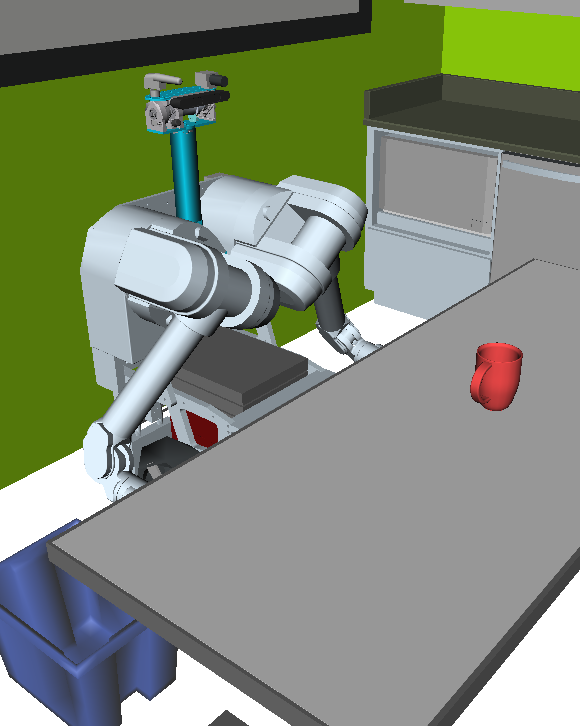
\includegraphics[width=0.185\linewidth]{figs/testherb-a.png}
   }
   \subfloat[Step 1, in $S_1$]{
      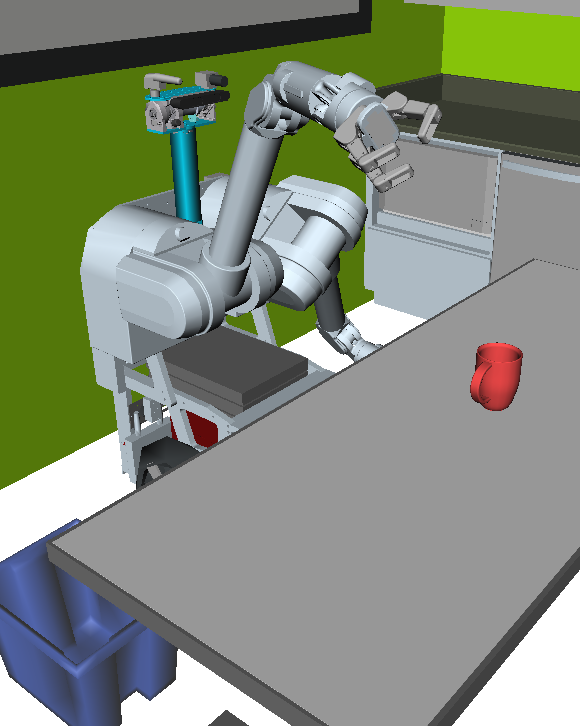
\includegraphics[width=0.185\linewidth]{figs/testherb-b.png}
   }
   \subfloat[Step 2, in $S_2$]{
      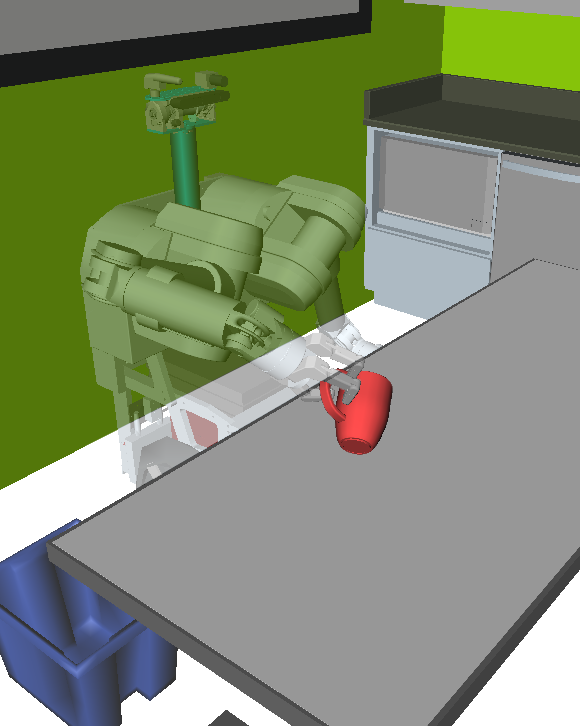
\includegraphics[width=0.185\linewidth]{figs/testherb-c.png}
   }
   \subfloat[Step 3, in $S_3$]{
      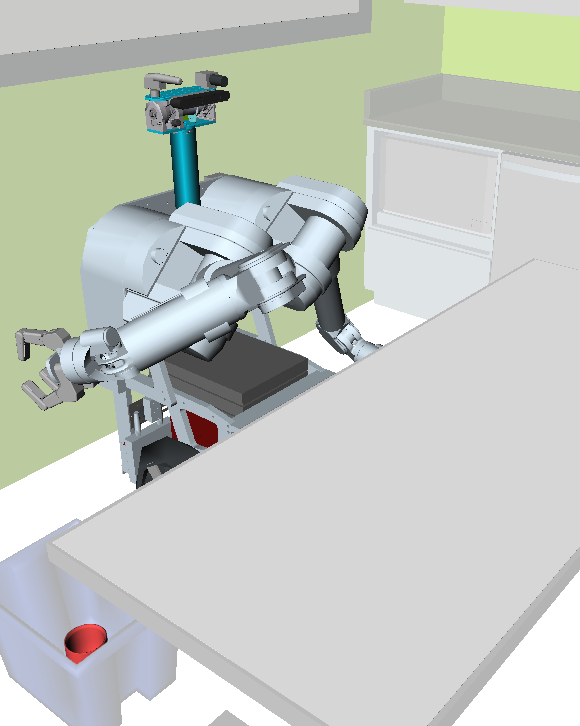
\includegraphics[width=0.185\linewidth]{figs/testherb-d.png}
   }
   \subfloat[Ending Configuration.]{
      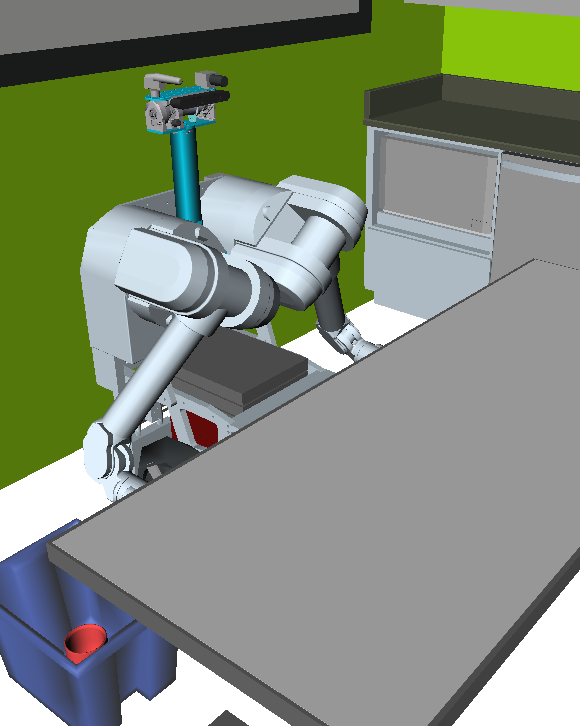
\includegraphics[width=0.185\linewidth]{figs/testherb-e.png}
   }

   \caption[][0.2in]{
     A home robot performing a three-step manipulation task.
     It must move from its home configuration
     to grasp the cup,
     transfer it to a drop location above the bin,
     and return home.
     Experimental results for the Family PRM
     are shown in Table~\ref{tab:family:testherb}}
   \label{fig:family:testherb-problem}
\end{figure*}

\begin{figure}
   \centering
   \includegraphics{build/multistep-prescribed/herbbin-g1ll}
   \caption{Example of planning over families for the HERB bin example
      problem (closest intermediate roots).
      RRT is red \protect\tikz{\protect\node[fill=red,draw=black]{};}.
      Individual LEMUR results are dashed
      (\protect\tikz{\protect\draw[thick,densely dotted] (0,0) -- (0.15,0.15);}),
      while Family-aware results are solid
      (\protect\tikz{\protect\draw[thick,solid] (0,0) -- (0.15,0.15);}),.
      Colors for the inner search algorithm are:
      \protect\tikz{\protect\node[fill=blue,draw=black]{};}\;IBiD,
      \protect\tikz{\protect\node[fill=purple,draw=black]{};}\;Heuristic IBiD,
      and \protect\tikz{\protect\node[fill=olive,draw=black]{};}\;A*.
      These results use $k_\gamma=1.0$ scaled by $\log(\log(n))/n$.
      }
\end{figure}

%\begin{figure}
%   \centering
%   \includegraphics{build/multistep-prescribed/herbbin-r0p9719o}
%   \caption{Example of planning over families for the HERB bin example
%      problem (closest intermediate roots).
%      RRT is red \protect\tikz{\protect\node[fill=red,draw=black]{};}.
%      Individual LEMUR results are dashed
%      (\protect\tikz{\protect\draw[thick,densely dotted] (0,0) -- (0.15,0.15);}),
%      while Family-aware results are solid
%      (\protect\tikz{\protect\draw[thick,solid] (0,0) -- (0.15,0.15);}),.
%      Colors for the inner search algorithm are:
%      \protect\tikz{\protect\node[fill=blue,draw=black]{};}\;IBiD,
%      \protect\tikz{\protect\node[fill=purple,draw=black]{};}\;Heuristic IBiD,
%      and \protect\tikz{\protect\node[fill=olive,draw=black]{};}\;A*.
%      These results use $R=2.0$ scaled by $1/n$.
%      }
%\end{figure}

\begin{figure}
   \centering
   \includegraphics{build/multistep-prescribed/herbbinnom-g1ll}
   \caption{Example of planning over families for the HERB bin example
      problem (nominated intermediate roots).
      RRT is red \protect\tikz{\protect\node[fill=red,draw=black]{};}.
      Individual LEMUR results are dashed
      (\protect\tikz{\protect\draw[thick,densely dotted] (0,0) -- (0.15,0.15);}),
      while Family-aware results are solid
      (\protect\tikz{\protect\draw[thick,solid] (0,0) -- (0.15,0.15);}),.
      Colors for the inner search algorithm are:
      \protect\tikz{\protect\node[fill=blue,draw=black]{};}\;IBiD,
      \protect\tikz{\protect\node[fill=purple,draw=black]{};}\;Heuristic IBiD,
      and \protect\tikz{\protect\node[fill=olive,draw=black]{};}\;A*.
      These results use $k_\gamma=1.0$ scaled by $\log(\log(n))/n$.
      }
\end{figure}

%\begin{figure}
%   \centering
%   \includegraphics{build/multistep-prescribed/herbbinnom-r0p9719o}
%   \caption{Example of planning over families for the HERB bin example
%      problem (nominated intermediate roots).
%      RRT is red \protect\tikz{\protect\node[fill=red,draw=black]{};}.
%      Individual LEMUR results are dashed
%      (\protect\tikz{\protect\draw[thick,densely dotted] (0,0) -- (0.15,0.15);}),
%      while Family-aware results are solid
%      (\protect\tikz{\protect\draw[thick,solid] (0,0) -- (0.15,0.15);}),.
%      Colors for the inner search algorithm are:
%      \protect\tikz{\protect\node[fill=blue,draw=black]{};}\;IBiD,
%      \protect\tikz{\protect\node[fill=purple,draw=black]{};}\;Heuristic IBiD,
%      and \protect\tikz{\protect\node[fill=olive,draw=black]{};}\;A*.
%      These results use $R=2.0$ scaled by $1/n$.
%      }
%\end{figure}

\begin{figure}
   \centering
   \includegraphics{build/multistep-prescribed/herbbookshelfnom-g1ll}
   \caption{Example of planning over families for the HERB bookshelf example
      problem, with nominated intermediate roots.
      RRT is red \protect\tikz{\protect\node[fill=red,draw=black]{};}.
      Individual LEMUR results are dashed
      (\protect\tikz{\protect\draw[thick,densely dotted] (0,0) -- (0.15,0.15);}),
      while Family-aware results are solid
      (\protect\tikz{\protect\draw[thick,solid] (0,0) -- (0.15,0.15);}),.
      Colors for the inner search algorithm are:
      \protect\tikz{\protect\node[fill=blue,draw=black]{};}\;IBiD,
      \protect\tikz{\protect\node[fill=olive,draw=black]{};}\;A*, and
      \protect\tikz{\protect\node[fill=cyan,draw=black]{};}\;LPA*.
      These results use $k_\gamma=1.0$ scaled by $\log(\log(n))/n$.
      }
\end{figure}

\begin{table*}[b]
   \begin{widepage}
   \centering
   \footnotesize
   \setlength{\tabcolsep}{3pt}
   \renewcommand{\arraystretch}{1.3}
   \begin{tabular}{|cc|r@{ }lr@{ }lr@{ }lr@{ }l|r@{ }lr@{ }lr@{ }lr@{ }l|r@{ }lr@{ }lr@{ }lr@{ }l|}
   \toprule
   \multirow{2}{*}{Relations} & \multirow{2}{*}{Cost}
     & \multicolumn{8}{c|}{$\lambda = 0$}
     & \multicolumn{8}{c|}{$\lambda = 0.5$}
     & \multicolumn{8}{c|}{$\lambda = 1$}
   \\
     &
     & Step & 1 & Step & 2 & Step & 3 & \multicolumn{2}{c|}{Total}
     & Step & 1 & Step & 2 & Step & 3 & \multicolumn{2}{c|}{Total}
     & Step & 1 & Step & 2 & Step & 3 & \multicolumn{2}{c|}{Total}
   \\ \midrule
   \multirow{2}{*}{None} & Plan
     &  6.16&s &  3.72&s &  2.38&s & 12.25&s
     &  5.52&s &  2.89&s &  2.12&s & 10.53&s
     &  3.39&s &  2.25&s &  2.12&s &  7.76&s
   \\
     & Exec
     & 14.22&rad &  8.51&rad &  4.23&rad & 26.97&rad
     & 15.07&rad & 10.60&rad &  4.23&rad & 29.89&rad
     & 15.07&rad & 10.60&rad &  4.23&rad & 29.89&rad
   \\ [1ex]
   Inter-Step & Plan
     &  6.40&s &  2.33&s &  0.86&s &  9.59&s
     &  5.40&s &  1.55&s &  0.91&s &  7.86&s
     &  3.38&s &  0.91&s &  0.30&s &  4.59&s
   \\
   (Sec.~\ref{subsec:family:dynamic-environments},~\ref{subsec:family:grasped-objects})
     & Exec
     & 14.22&rad &  8.51&rad &  4.23&rad & 26.97&rad
     & 15.07&rad & 12.21&rad &  4.23&rad & 31.51&rad
     & 15.07&rad & 12.21&rad &  7.11&rad & 34.40&rad
   \\ [1ex]
   Self-Checked & Plan*
     &  3.54&s &  2.23&s &  1.17&s & 6.94&s
     &  2.99&s &  1.77&s &  1.16&s & 5.92&s
     &  1.47&s &  1.22&s &  1.16&s & 3.85&s
   \\
   (Sec.~\ref{subsec:family:cached-self-valid}) & Exec
     & 14.22&rad &  8.51&rad &  4.23&rad & 26.96&rad
     & 14.22&rad & 10.06&rad &  4.23&rad & 28.51&rad
     & 14.22&rad & 10.60&rad &  4.23&rad & 29.05&rad
   \\ [1ex]
   \multirow{2}{*}{Both} & Plan*
     &  3.25&s &  1.79&s &  0.90&s & 5.94&s
     &  2.88&s &  1.55&s &  0.92&s & 5.35&s
     &  1.47&s &  1.88&s &  0.31&s & 3.66&s
   \\
     & Exec
     & 14.22&rad &  8.51&rad &  4.23&rad & 26.96&rad
     & 14.22&rad &  8.51&rad &  4.23&rad & 26.96&rad
     & 14.22&rad &  9.64&rad &  6.36&rad & 30.22&rad
   \\ 
   \bottomrule
   \end{tabular}
   \caption[][-0.1in]{Home robot manipulation task results.
     The entry with no relations and $\lambda=0$ is equivalent
     to the LazyPRM.
     These are old results.}
   \label{tab:family:testherb}
   \end{widepage}
\end{table*}

\begin{figure}
   \centering
   \hspace{0.2cm}
   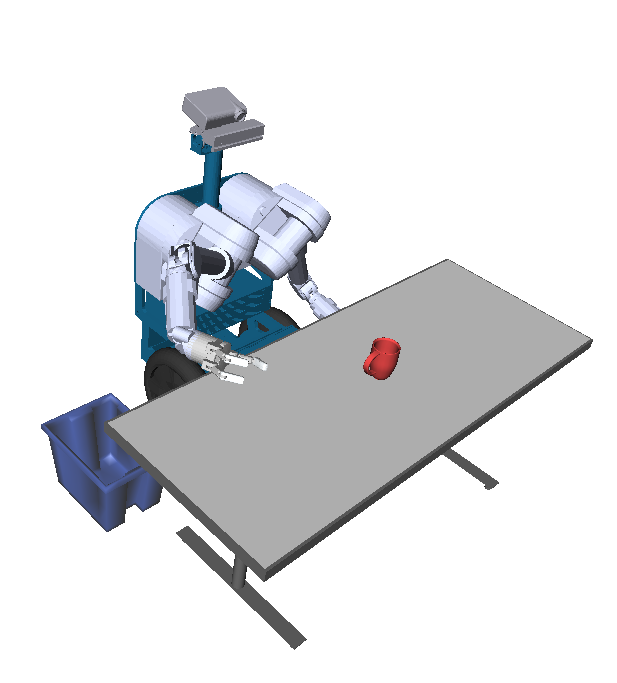
\includegraphics[width=2.7cm]{figs/herbarmmultithread/herbarmmultithread-step0.png}%
   \;
   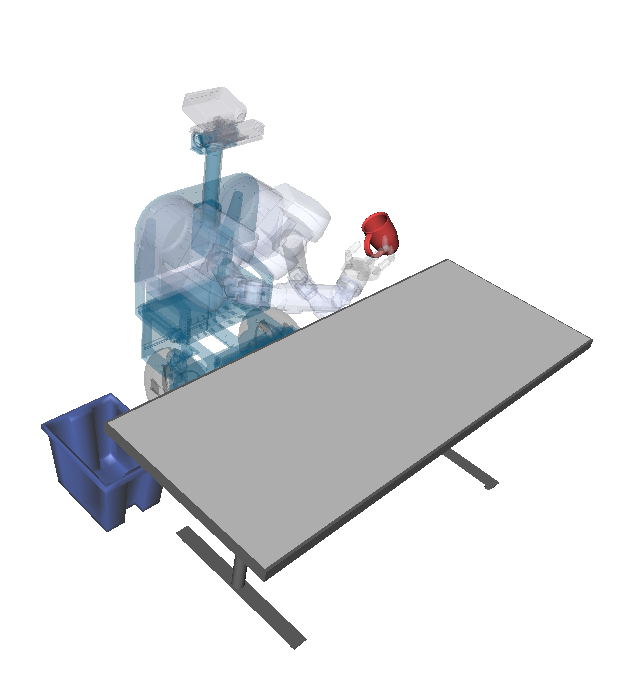
\includegraphics[width=2.7cm]{figs/herbarmmultithread/herbarmmultithread-step1.png}%
   \;
   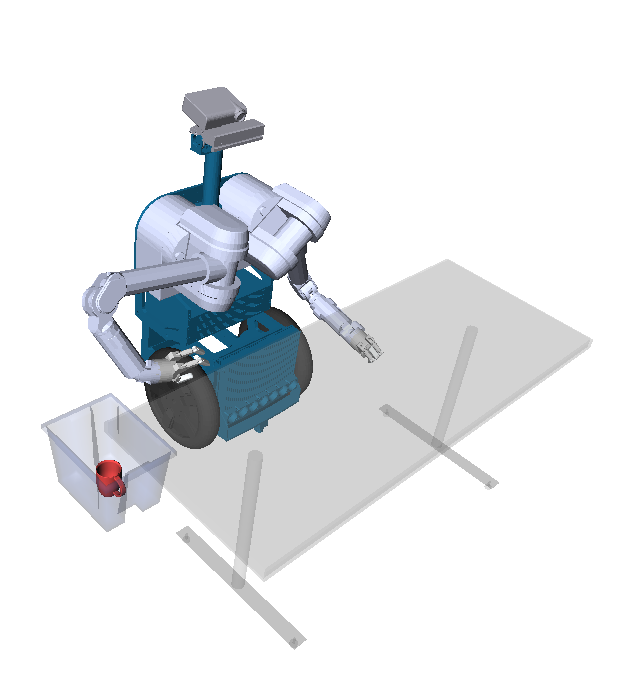
\includegraphics[width=2.7cm]{figs/herbarmmultithread/herbarmmultithread-step2.png}%
   
   \includegraphics{build/herbarmmultithread/master-fig}
   \caption[]{
      Results from a motion planning experiment for manipulation
      planning in which the robot must move to grasp the mug
      and place it into a bin at its side
      before returning to its initial configuration.
      In the course of planning the first step to the grasp point,
      the planner has discovered a number of edges known to be
      valid.
      After the grasp, the robot must find a motion to transfer the
      mug -- any edges known to be valid in the previous step
      can be used after only checking that the grasped mug does not
      collide with the environment.
      Compared with a sequence of single-query calls to LEMUR
      with model $\mathcal{C}_{\ms{simple}}$
      \protect\tikz{\protect\node[fill=black!80,draw=black]{};},
      LEMUR armed with the $\mathcal{M}_{\ms{family}}$ ensemble
      cost model
      \protect\tikz{\protect\node[fill=cyan,draw=black]{};}
      can guide the planner to use edges that are less
      expensive to validate.}
   \label{fig:family:herbarmmultithread-master}
\end{figure}

Here's some notes on the workcell example:

\begin{verbatim}
workcell basic (independent) atoms:
 (1) (robot) x (self+staticenv)
 (2) (robot) x (sheetstart)
 (3) (robot) x (sheetregrasp)
 (4) (robot) x (sheetend)
 (5) (robotgrabtop-sheetmidside2flat) x (self+staticenv)
 (6) (robotgrabtop-sheetside1flat) x (self+staticenv)
 (7) (robotgrabtop-sheetside1bent) x (self+staticenv)
 (8) (robotgrabbottom-sheetmidside1bent) x (self+staticenv)
 (9) (robotgrabbottom-sheetside2flat) x (self+staticenv)
(10) (robotgrabbottom-sheetside2bent) x (self+staticenv)

each problem step is built of atoms:
 step AB = (1) n (2)
 step BC = (1) n (5) n (6)
 step CD = (1) n (5) n (6)
 step EF = (1) n (5) n (7)
 step FG = (1) n (3)
 step GH = (1) n (8) n (9)
 step IJ = (1) n (8) n (10)
 step JA = (1) n (4)

FamilyUtilityChecker reports 17 vars (makes sense)

2**10 =  1024 truth table rows
\end{verbatim}






\section{Application: Caching Invariant Geometry}
\label{subsec:family:cached-self-valid}

\paragraph{Cached Self-Collision-Checked Roadmaps}
Self-collision checking is a potentially expensive component to
articulated motion planning;
in contrast to environment checking,
it is fundamentally quadratic in the number of moving links.
Further, pairs of links to be checked
tend to be relatively close to each other,
reducing the effeciveness of broad-phase approaches.

Leven and Hutchinson \citep{leven2000changing}
introduced the concept of a pre-cached roadmap consisting of
configurations and paths already known to be valid w.r.t.
self-collision.
As a type of invariant in $\mathcal{C}$,
this can be seen as a particular instance of family motion planning.
See Fig.~\ref{fig:family:self-collision-example}.

\begin{figure*}
   \centering   
   \includegraphics{build/family-sq-caching/pvxs}
   \caption[]{LEMUR single-query results on several HERB problems,
      all using baked calls.
      Traces are LEMUR
      (\protect\tikz{\protect\draw[thick,black] (0,0) -- (0.15,0.15);}),
      the family motion planner (no caching)
      (\protect\tikz{\protect\draw[thick,blue] (0,0) -- (0.15,0.15);}),
      or the family motion planner with self-checked caching
      (\protect\tikz{\protect\draw[thick,green] (0,0) -- (0.15,0.15);}).}
\end{figure*}





\section{Application: Exploiting Conservative Geometric Approximations}
\label{subsec:family:broad-phase}

The family formulation also enables motion planners to
reason directly about different robot or environment models.
For example, consider two geometric robot models,
one with high quality (e.g. from a CAD program),
and one hand-tuned ``padded'' model consisting of 
a small number of simple conservative bounding volumes.
The $\mathcal{C}$-subsets derived from these models
are related by $R_{\ms{padded}} \subseteq R_{\ms{CAD}}$.
Collision checkers currently use a similar approach internally
to speed up collision checks (see Fig.~\ref{fig:family:broad-phase}.
and Fig~\ref{fig:family:broad-phase-2d}).

See Figure~\ref{fig:family:broad-phase-2d}
for a simple example with integrated broad-phase collision checking
as described in Section~\ref{subsec:family:broad-phase}.

\begin{figure*}[b]
   \centering
   
   \subfloat[
      A single-set planner testing simply for membership in
      $\mathcal{C}_{\mbox{\scriptsize free}}$
      treats a collision validity checker as a
      ``black box.''
      Internally,
      modern checkers first employ an inexpensive broad-phase check
      using a low-dimensional conservative representation
      to quickly identify non-colliding bodies before
      resorting to an expensive narrow-phase check.
   ]{%
      \includegraphics{build/broadphase-single}%
   }%
   \quad%
   \subfloat[
      A family motion planner can explicitly reason about the
      conservative nature of the broad-phase check.
      This allows it to defer some narrow phase checks
      (often indefinitely)
      and instead prefer paths that require fewer expensive checks.
   ]{%
      \includegraphics{build/broadphase-multi}%
   }
   
   \caption[][0.0in]{Collision validity checking is a commonly used
     indicator function.
     The family formulation allows an intelligent planner to
     reach inside the checker's ``black box'' and reduce the number
     of costly narrow-phase checks.
     Resulting paths tend to be cheaper to compute and
     stay further from obstacles.}
   \label{fig:family:broad-phase}
\end{figure*}

% this is the broad phase bean figure
\begin{figure}
   \centering

   % left side
   \subfloat[Paths with lambda=0][%
      \centering
      Paths with $\lambda = 0$\par
      Average length: 733.0\par
      Average check cost: 7219.5
   ]{
      \includegraphics[width=0.45\textwidth]
      {figs/bean-allpaths-lambda0.png}
   }
   % right side
   \subfloat[Paths with lambda=1][%
      \centering
      Paths with $\lambda = 1$\par
      Average length: 836.5\par
      Average check cost: 4692.6
   ]{
      \includegraphics[width=0.45\textwidth]
      {figs/bean-allpaths-lambda1.png}
   }
   \\
   \subfloat[Paths with lambda=0][%
      \centering
      Paths with $\lambda = 0$\par
      Average length: 733.0\par
      Average check cost: 2685.7
   ]{
      \includegraphics[width=0.45\textwidth]
      {figs/bean-allpaths-padded-lambda0.png}
   }
   % right side
   \subfloat[Paths with lambda=1][%
      \centering
      Paths with $\lambda = 1$\par
      Average length: 907.1\par
      Average check cost: 1064.5
   ]{
      \includegraphics[width=0.45\textwidth]
      {figs/bean-allpaths-padded-lambda1.png}
   }

   \caption{A simple 2D example of the Family PRM using
     a broad-phase check.
     Checking for collision with the grey box is 10x less expensive
     than with the actual black obstacle.}
     %\cdnote{I need to talk about this in the text.}}
   \label{fig:family:broad-phase-2d}
\end{figure}






\section{Application: Dynamic Environments}

\paragraph{Dynamic Environments.}
\label{subsec:family:dynamic-environments}

\begin{figure}
   \centering

   \begin{minipage}{.6\textwidth}
      \begin{tikzpicture}
      \tikzset{>=latex} % arrow heads
      \node[anchor=south west,inner sep=0] at (0,0)
        {\includegraphics[width=0.8\textwidth]{figs/chimp-voxels-delta.png}};

      \node[draw,inner sep=3pt,fill=white,fill opacity=0.9,align=center]
        (debrislab) at (0.7,1.0) {Debris object\\removed};
      \node[circle,inner sep=2,draw,fill=white] (debris) at (2.2,2.9) {};
      \draw[draw=black, double=white, double distance=1pt, line width=1pt]
        (debrislab.north) -- (debris);
        
      \node[draw,inner sep=3pt,fill=white,fill opacity=0.9,align=center]
        (addlab) at (5.0,2.0) {Additional\\voxels seen};
      \node[circle,inner sep=2,draw,fill=white] (added) at (4.4,5.0) {};
      \draw[draw=black, double=white, double distance=1pt, line width=1pt]
        (addlab.north) -- (added);
        
      \end{tikzpicture}
   \end{minipage}%
   \,%
   \begin{minipage}{.35 \textwidth}
      \includegraphics{build/retroactive-a}
      
      \includegraphics{build/retroactive-b}
   \end{minipage}

   \caption{
      Structured or unstructured dynamic environments
      can be represented as a family problem
      (see Section~\ref{subsec:family:dynamic-environments}).
      
      \vspace{0.05in}
      \noindent
      (Left) A disaster response robot maintains a
      dynamic unstructured environment model
      using coarse voxels
      (scene data from a debris-clearing task at a
      recent disaster response competition).
      Since the last planning query,
      voxels have been added (green) and removed (red).
      
      \vspace{0.05in}
      \noindent
      (Right) $\mathcal{C}$-subsets and relations
      can be added retroactively.
      Here, the graph for an initial query is checked w.r.t $S_1$.
      After environment changes,
      $S_1$ is redefined in terms of the $\mathcal{C}$-subsets
      derived from the set of common, added, and removed elements,
      allowing for reuse on a query in $S_2$.
      Here,
      the planner need only check existing path segments
      against added voxels in order to reuse them for the current query.}
   \label{fig:family:dynamic-environments}
\end{figure}

The sensors on most articulated robots allow them to maintain
dynamic environment models to track changing collision geometry.
These models might be
structured (e.g. recognizing objects with known models)
or unstructured (e.g. occupancy models).
In both cases,
even in a changing world,
there are often areas that are fixed between planning queries.

Prior work (e.g. \citep{jaillet2004dynamicprm})
leverages this by imposing a dichotomy between
\emph{fixed} and \emph{moving} components of $\mathcal{C}$.
Our formulation extends this to an arbitrary number of such labels,
including ones defined retroactively (i.e. during planning;
see Fig.~\ref{fig:family:dynamic-environments}).
By explicitly labeling such areas in workspace
(and leveraging the \emph{set containment} property
\citep{newmanbranicky1991cspacetransforms}),
we can represent this structure as a family motion planning problem.


\section{Implementation Details}

We provide an implementation for the
OpenRAVE \citep{diankov2010openrave}
virtual kinematic planning environment
which automatically discovers $\mathcal{C}$-subsets
in manipulation tasks.




\section{Other Stuff}

\pgfplotstableread{
barname mean error
RRTConnect 2.56378257751494 0.1819787187133847
LazyPRM(*) 2.59627093791926 0.07645708288005078
LEMUR(SQ) 1.95654549121872 0.04821756844687192
LEMUR(MQ) 1.5911829090115797 0.03471955055186312
}{\datalemurherbbin}

\begin{figure}
   \centering
   \begin{tikzpicture}
      \begin{axis}[
         width=6.0cm,
         height=4.0cm,
         xbar,
         bar width=12,
         xmin=0,
         enlarge y limits={abs=0.45cm},
         %xmin=0,xmax=95,
         %xtick pos=bottom,
         %symbolic y coords={E, F, R, A, B, W, P},
         yticklabels from table={\datalemurherbbin}{barname},
         ytick=data,
         ytick pos=left,
         xmajorgrids,
         %xmajorticks=false,
         ticklabel style={font=\footnotesize},
         xlabel={\footnotesize{Planning time $p$ (s)}},
         xlabel near ticks,
         ] 
      %\node[circle,fill=white,inner sep=1pt,text=black!40] at (axis cs:40,-5.6) {\scriptsize 40};
      %\node[circle,fill=white,inner sep=1pt,text=black!40] at (axis cs:60,-5.6) {\scriptsize 60};
      %\node[circle,fill=white,inner sep=1pt,text=black!40] at (axis cs:80,-5.6) {\scriptsize 80};
      \addplot[color=black,fill=black!20,error bars/.cd,x dir=both,x explicit]
         table[y expr=-\coordindex,x=mean,x error expr=\thisrow{error}]
         {\datalemurherbbin};
      \end{axis}
   \end{tikzpicture}
   \caption{LEMUR Herbbin, $\lambda = 1$}
\end{figure}

\pgfplotstableread{
barname mean error
RRTConnect 17.735649337767864 0.8572182241158215
LazyPRM(*) 11.02914777755716 0.2718847854283968
LEMUR(SQ) 8.987455253601558 0.22683157494511255
LEMUR(MQ) 5.995352478027379 0.23607184395127515
}{\datalemurworkcell}

\begin{figure}
   \centering
   \begin{tikzpicture}
      \begin{axis}[
         width=6.0cm,
         height=4.0cm,
         xbar,
         bar width=12,
         xmin=0,
         enlarge y limits={abs=0.45cm},
         %xmin=0,xmax=95,
         %xtick pos=bottom,
         %symbolic y coords={E, F, R, A, B, W, P},
         yticklabels from table={\datalemurworkcell}{barname},
         ytick=data,
         ytick pos=left,
         xmajorgrids,
         %xmajorticks=false,
         ticklabel style={font=\footnotesize},
         xlabel={\footnotesize{Planning time $p$ (s)}},
         xlabel near ticks,
         ] 
      \node[circle,fill=white,inner sep=1pt,text=black!40] at (axis cs:40,-5.6) {\scriptsize 40};
      \node[circle,fill=white,inner sep=1pt,text=black!40] at (axis cs:60,-5.6) {\scriptsize 60};
      \node[circle,fill=white,inner sep=1pt,text=black!40] at (axis cs:80,-5.6) {\scriptsize 80};
      \addplot[color=black,fill=black!20,error bars/.cd,x dir=both,x explicit]
         table[y expr=-\coordindex,x=mean,x error expr=\thisrow{error}]
         {\datalemurworkcell};
      \end{axis}
   \end{tikzpicture}
   \caption{LEMUR Workcell, $\lambda = 1$}
\end{figure}

% data over 84 data points
% there are 85 PlanToNamedConfiguration planning requests in
% my planning_queries/yaml/* directory;
% i paired them up, and these are the numbers across all pairs
\pgfplotstableread{
barname mean stderror95
FamilyFirst 0.3858953203473929 0.011569714605374383
FamilySecond 0.18286271038508334 0.0070175681823757274
}{\datalemurtableclear}

\begin{figure}
   \centering
   \begin{tikzpicture}
      \begin{axis}[
         width=6.0cm,
         height=3.0cm,
         xbar,
         bar width=12,
         xmin=0,
         enlarge y limits={abs=0.45cm},
         %xmin=0,xmax=95,
         %xtick pos=bottom,
         %symbolic y coords={E, F, R, A, B, W, P},
         yticklabels from table={\datalemurtableclear}{barname},
         ytick=data,
         ytick pos=left,
         xmajorgrids,
         %xmajorticks=false,
         ticklabel style={font=\footnotesize},
         xlabel={\footnotesize{Planning time $p$ (s)}},
         xlabel near ticks,
         ] 
      %\node[circle,fill=white,inner sep=1pt,text=black!40] at (axis cs:40,-5.6) {\scriptsize 40};
      %\node[circle,fill=white,inner sep=1pt,text=black!40] at (axis cs:60,-5.6) {\scriptsize 60};
      %\node[circle,fill=white,inner sep=1pt,text=black!40] at (axis cs:80,-5.6) {\scriptsize 80};
      \addplot[color=black,fill=black!20,error bars/.cd,x dir=both,x explicit]
         table[y expr=-\coordindex,x=mean,x error expr=\thisrow{stderror95}]
         {\datalemurtableclear};
      \end{axis}
   \end{tikzpicture}
   \caption{Family Tableclear, $\lambda = 0$}
\end{figure}

%\cdnote{%
%Special case of this is if objects are disappearing.
%Relation to occupancy grid representations of workspace
%(for deltas, conservative approxs, etc).}

% OTHER POTENTIAL APPLICATIONS:
%
%\subsubsection*{Conservative Bounding Volumes for Different Grasps}
%
%\subsubsection*{Conservative Bounding Volumes for Hypothesized Objects}
%
%There's a sweet ICRA paper here.
%
%\subsubsection*{Dual Arm Stuff}
%
%I think this is related.
%
%Check right arm against gian left side box, etc.
%
%\subsubsection*{Dimensionality Reduction}
%
%The Handey \cite{lozanoperez1987handey} robot
%assumed a box that contained the wrist links at a range of DOF values.
%
%\subsubsection*{Dual-Arm Stuff}
%
%This is very similar to dimensionality reduction.
%
%Loose coupling between arms.
%
%Separate roadmaps for each arm.
%
%Investigate this family structure.
